\documentclass{article}
\usepackage{graphicx}
\usepackage{float}
\usepackage{epstopdf}

\begin{document}
\begin{center}
CMPE245 Project 1
\end{center}
Chien-Pin Chen\\
06/07/2016\\

\noindent In Extend Kalman Filter, the system model (equation 1 and 2) of the project 1 could refer to:

\begin{equation}
	\underline{x}_{k + 1}  = \underline{f}_k (\underline{x}_k ,\underline{w}_k )
\end{equation}

then, for computing, I could set:
\begin{equation}
	\begin{array}{l}
	\underline{x}_{k + 1}  = \underline{f}_k (\hat{\underline{x}}_k ,0) \\ 
	 \underline{x}_{k + 1}  = \left[ {\begin{array}{*{20}c}
	   {\underline{x}_1 (k + 1)}  \\
	   {\underline{x}_2 (k + 1)}  \\
	   {\underline{x}_3 (k + 1)}  \\
	   {\underline{x}_4 (k + 1)}  \\
	\end{array}} \right] = \left[ {\begin{array}{*{20}c}
	   {\underline{x}_1 (k) + \Delta t \cdot x_3 \cos x_4 }  \\
	   {\underline{x}_2 (k) + \Delta t \cdot x_3 \sin x_4 }  \\
	   {\underline{x}_3 (k)}  \\
	   {\underline{x}_4 (k)}  \\
	\end{array}} \right] \\ 
	 \end{array}
\end{equation}
\begin{equation}
	\underline{\Phi} _k  = \frac{{\partial \underline{f}_k (\hat{\underline{x}}_k ,0)}}{{\partial \underline{x}_k }} = \left[ {\begin{array}{*{20}c}
	   0 & 0 & {\Delta t \cdot \cos x_4 } & { - \Delta t \cdot x_3 \sin x_4 }  \\
	   0 & 0 & {\Delta t \cdot \sin x_4 } & {\Delta t \cdot x_3 \cos x_4 }  \\
	   0 & 0 & 1 & 0  \\
	   0 & 0 & 0 & 1  \\
	\end{array}} \right]
\end{equation}
\begin{equation}
	\underline{\Gamma}_k  = \frac{{\partial \underline{f}_k (\hat{\underline{x}}_k ,0)}}{{\partial \underline{w}_k }} = \left[ {\begin{array}{*{20}c}
	   {\begin{array}{*{20}c}
	   0  \\
	   0  \\
	   {\delta _v \sqrt {dt} }  \\
	   0  \\
	\end{array}} & {\begin{array}{*{20}c}
	   0  \\
	   0  \\
	   0  \\
	   {\delta _w \sqrt {dt} }  \\
	\end{array}}  \\
	\end{array}} \right]
\end{equation}
\begin{equation}
\underline{Q}=\left[ \begin{array}{cc}
1 & 0 \\ 
0 & 1
\end{array}\right]  
\end{equation}
In equation (2), (3), and (4), because the measure data are took every 10 frames (30 frames per second), 
$\delta t$ and $dt$ are set as $\frac{1}{3}$. In addition, in equation (2) of the project 1, because $\xi_v (t)$ 
and $\xi_\theta (t)$ are zero-mean white noises, I set $\delta_v$ and $\delta_\theta$ (in my equation 4) as 
zero at first. Then, I will tune those values according to the result of extended Kalman filter later.\\ 
Next, the measurement model (the equation 3) of the project 1 could refer to:
\begin{equation}
	\underline{y}_k = \underline{h}_k(\underline{x}_k) + \underline{v}_k
\end{equation}
then, for computing, I could set:
\begin{equation}
	\underline{{\rm H}}_k  = \frac{{\partial \underline{h}_k (\hat{\underline{x}}_k (-))}}{{\partial x_k }} = \left[ {\begin{array}{*{20}c}
	   {\begin{array}{*{20}c}
	   1 & 0 & 0 & 0  \\
	\end{array}}  \\
	   {\begin{array}{*{20}c}
	   0 & 1 & 0 & 0  \\
	\end{array}}  \\
	\end{array}} \right]
\end{equation}
\begin{equation}
	R = \left[ {\begin{array}{*{20}c}
	   {{\mathop{\rm var}} \{ x_m \} } & 0  \\
	   0 & {{\mathop{\rm var}} \{ y_m \} }  \\
	\end{array}} \right]
\end{equation}
In equation 8, $var\{x_m\}$ and $var\{y_m\}$ are the variance of the measurement of robot position. Because the 
provided data are measured from the video of moving epuck, the variance of robot position will depend on the 
quality of the video. The following steps describe how to compute the variance of  any position in the video. First,
 I use the movie player in MATLAB to load 'Project1Movie.AVI' and exported the first frame to Image tool (also a 
 toolbox in MATLAB). In the first frame, I measure how many pixels between two back lights, and this number (28.75 
 in figure 1) divide the real distance between two back lights, which is 46 mm, is 1.6 mm per pixel. Because the 
 position of LED light in the video is blurred, it is the noise for the measure data. Then, from figure 1, I get the range 
 of blurred LED light is 7.1 pixel  (11.36 mm), and I assume it is 3 times std. of the Gaussian distribution the noise of
 LED light. Therefore, I get the standard deviation of the noise any position in the video is 0.3786, and the variance is 
 0.1434. 
 \begin{figure}[H]
	 \begin{center}
	 	\includegraphics[width=\textwidth]{measure_noise.jpg}
	 	\caption{Compute the noise of the video.}
	 \end{center}
 \end{figure}

In the prediction step of Extended Kalman filter (EKF), I use following equations for discrete time model:
\begin{eqnarray}
\underline{\hat{x}}_{k + 1}(-)  = \underline{\hat{f}}_k (\underline{\hat{x}}_k ,0)\\
\underline{P}_{k + 1} ( - ) = \underline{\Phi}_k \underline{P}_k \underline{\Phi}_k^T + \underline{\Gamma}_k Q \underline{\Gamma}_k^T 
\end{eqnarray}
For initial guess of $\underline{\hat{x}}_0$, I use the first element of the measurement data as $E\{x(0)\}$ and $E\{y(0)\}$, 
and also use the second element with the first to compute initial velocity ($E\{v(0)\}$) and heading angle ($E\{\theta(0)\}$):
\begin{equation}
\underline{\hat{x}}_0  = \left[ {\begin{array}{*{20}c}
   {x_m (0)}  \\
   {y_m (0)}  \\
   {\sqrt {(x_m (1) - x_m (0))^2  + (y_m (1) - y_m (0))^2 } }  \\
   {\tan ^{ - 1} (\frac{{(y_m (1) - y_m (0))}}{{(x_m (1) - x_m (0))}})}  \\
\end{array}} \right]
\end{equation} 
For initial guess of $\underline{\hat{P}}_0$, because the robot position is measured by the average of the 
position of three LED light, which are affected by the variance of the noise. Also, my initial expected value of 
velocity and heading angle is acquired from initial robot position, so I set the covariance of $v_0$ and $\theta_0$
according to the variance of the robot position.  The following is how I compute the state covariance:
\begin{equation}
	\begin{array}{l}
	 {\mathop{\rm cov}} \{ x,x\}  = P_{11}  = P_{22}  = 3 \times (light\_noise^2 )/9 \\ 
	 {\mathop{\rm cov}} \{ \theta ,\theta \}  = P_{44}  = (10{\raise0.7ex\hbox{${pi}$} \!\mathord{\left/
	 {\vphantom {{pi} {180}}}\right.\kern-\nulldelimiterspace}
	\!\lower0.7ex\hbox{${180}$}})^2  \\ 
	 P_{13}  = P_{14}  = P_{23}  = P_{24}  = P_{11}  \\ 
	 \underline{\hat{P}}_0  = \left[ {\begin{array}{*{20}c}
	   {P_{11} } & 0 & {P_{13} } & {P_{14} }  \\
	   0 & {P_{22} } & {P_{23} } & {P_{24} }  \\
	   {P_{13} } & {P_{23} } & {2{\raise0.7ex\hbox{${P_{11} }$} \!\mathord{\left/
	 {\vphantom {{P_{11} } {\Delta t^2 }}}\right.\kern-\nulldelimiterspace}
	\!\lower0.7ex\hbox{${\Delta t^2 }$}}} & 0  \\
	   {P_{14} } & {P_{24} } & 0 & {P_{44} }  \\
	\end{array}} \right] \\ 
	 \end{array}
\end{equation}

Next, I use following equations in the update step of EKF:
\begin{eqnarray}
	\underline{K}_{k + 1}  = \underline{P}_{k + 1} ( - )\underline{H}_{k + 1}^T (\underline{H}_{k + 1} \underline{P}_{k+ 1} ( - )\underline{H}_{k + 1}^T  + \underline{R}_{k + 1} )^{ - 1} \\
	\underline{\hat{x}}_{k + 1}  = \underline{\hat{x}}_{k + 1} ( - ) + \underline{K}_{k + 1} (\underline{y}_{k + 1}  - \underline{h}_{k + 1} (\underline{\hat{x}}_{k + 1} ( - )))\\
	\underline{P}_{k + 1}  = (I - \underline{K}_{k + 1} \underline{H}_{k + 1} )\underline{P}_{k + 1} ( - )
\end{eqnarray}
After updating, do another extended Kalman filter with next measurement data $Z(k)$, which is provided in XYData\_cm.csv file.\\
For second order Kalman filter, I use following equations for prediction step:
\begin{eqnarray}
	\underline{\hat{x}}_{k + 1}  = \underline{f}_k (\underline{\hat{x}}_k ,0) + \underline{b}_k\\
	\underline{x}_{k + 1}  = \left[ {\begin{array}{*{20}c}
	   {\underline{x}_1 (k + 1)}  \\
	   {\underline{x}_2 (k + 1)}  \\
	   {\underline{x}_3 (k + 1)}  \\
	   {\underline{x}_4 (k + 1)}  \\
	\end{array}} \right] = \left[ {\begin{array}{*{20}c}
	   {\underline{x}_1 (k) + \Delta t \cdot x_3 \cos x_4 }  \\
	   {\underline{x}_2 (k) + \Delta t \cdot x_3 \sin x_4 }  \\
	   {\underline{x}_3 (k)}  \\
	   {\underline{x}_4 (k)}  \\
	\end{array}} \right] + \underline{b}_k \\
	\underline{b}_k  = \frac{1}{2}\sum\limits_{i = 1}^n {e_i \left( {\frac{1}{2}tr\left[ {F_k^i P_k } \right] + \frac{1}{2}tr\left[ {G_k^i P_k } \right]} \right)} ,e_i  \in R^n\\ 
	\underline{P}_{k + 1} ( - ) = \underline{\Phi}_k \underline{P}_k \underline{\Phi}_k^T + \underline{\Gamma}_k Q \underline{\Gamma}_k^T
\end{eqnarray}
For $\underline{b}_k$ of equation 18, $F_k^i$ is the element of hessian of $\underline{f}_k(\underline{\hat{x}}_k, 0)$ w.r.t $\underline{x}_k$. Therefore, I could 
compute as:
\begin{equation}
\begin{array}{l}
 F_k^1  = \frac{{\partial ^2 f_k^1 (\hat x_k ,0)}}{{\partial ^2 x_k }} = \frac{\partial }{{\partial x_k }}\left[ {\begin{array}{*{20}c}
   0  \\
   0  \\
   {\Delta t \cdot \cos x_4 }  \\
   { - \Delta t \cdot x_3 \sin x_4 }  \\
\end{array}} \right] = \left[ {\begin{array}{*{20}c}
   0 & 0 & 0 & 0  \\
   0 & 0 & 0 & 0  \\
   0 & 0 & 0 & { - \Delta t \cdot \sin x_4 }  \\
   0 & 0 & { - \Delta t \cdot \sin x_4 } & { - \Delta t \cdot x_3 \cos x_4 }  \\
\end{array}} \right] \\ 
 F_k^2  = \frac{{\partial ^2 f_k^2 (\hat x_k ,0)}}{{\partial ^2 x_k }} = \frac{\partial }{{\partial x_k }}\left[ {\begin{array}{*{20}c}
   0  \\
   0  \\
   {\Delta t \cdot \sin x_4 }  \\
   {\Delta t \cdot x_3 \cos x_4 }  \\
\end{array}} \right] = \left[ {\begin{array}{*{20}c}
   0 & 0 & 0 & 0  \\
   0 & 0 & 0 & 0  \\
   0 & 0 & 0 & {\Delta t \cdot \cos x_4 }  \\
   0 & 0 & {\Delta t \cdot \cos x_4 } & { - \Delta t \cdot x_3 \sin x_4 }  \\
\end{array}} \right] \\ 
 F_k^3  = \frac{{\partial ^2 f_k^3 (\hat x_k ,0)}}{{\partial ^2 x_k }} = \frac{\partial }{{\partial x_k }}\left[ {\begin{array}{*{20}c}
   0  \\
   0  \\
   1  \\
   0  \\
\end{array}} \right] = \left[ {0_{4 \times 4} } \right],F_k^4  = \frac{{\partial ^2 f_k^4 (\hat x_k ,0)}}{{\partial ^2 x_k }} = \frac{\partial }{{\partial x_k }}\left[ {\begin{array}{*{20}c}
   0  \\
   0  \\
   0  \\
   0  \\
\end{array}} \right] = \left[ {0_{4 \times 4} } \right] \\ 
 \end{array}
\end{equation}
And, $G_k^i$ is the element of hessian of $\underline{f}_k(\underline{\hat{x}}_k, 0)$ w.r.t $\underline{w}_k$. 
Because it is second partial derivative to $\underline{w}_k$, all of $G_k^i$ are matrices with all zero. \\
For update step of the second order Kalman filter, I use following eqauation:
\begin{eqnarray}
P_{k + 1}  = P_{k + 1} ( - ) - P_{k + 1} ( - )H_{_{k + 1} }^T \left[ {H_{k + 1} P_{k + 1} ( - )H_{_{k + 1} }^T  + R_{k + 1}  + S_{k + 1} } \right]^{ - 1} H_{k + 1} P_{k + 1} ( - ) \\
K_{k + 1}  = P_{K + 1} H_{k + 1}^T (R_{k + 1}  + S_{k + 1} )^{ - 1} \\
\underline{\hat x}_{k + 1}  = \underline{\hat x}_{k + 1} ( - ) + K_{k + 1} (y_{k + 1}  - h_{k + 1} (\underline{\hat x}_{k + 1} ( - ))) + s_{k + 1}
\end{eqnarray}
Also, in my kalman filter loop, I also use the position in previous loop to get the reasonable measurement velocity in 
order to compare with the expected velocity I get from the EKF. 
Now, with needed equations and initial values, I could start to run extended Kalman filter and second order filter, 
First, I run EKF with $\delta_v^2=1$ and $\delta_\theta^2=1$. The result is shown in figure 2. From the result of 
the robot position, it shows that the value of $\delta_v^2$ and $\delta_\theta^2$ are too large, so my predicted 
position almost match with the measurement data. Although the result of robot velocity seems fine, the result 
heading angle is not match the $\alpha$ angle (from HeadingAngle\_rad.csv) well. The expected heading angle is not
smooth at 12-15 second.\\
Next, in order to get better result of the heading angle, I use smaller values, such as $\delta_v^2=0.05$ and 
$\delta_\theta^2=0.01$. From the result of figure 3, though the expected robot position is not follow the 
measurement data well, the expected heading angle is more smooth and follow the changing of $\alpha$ angle.
Also, the expected velocity smoothly changing, but it do not diverge from the measurement velocity. 
 \begin{figure}[H]
	 \begin{center}
	 	\includegraphics[width=\textwidth]{EKF_v1_w1.eps}
	 	\caption{The result of EKF with $\delta_v^2=1$ and $\delta_\theta^2=1$.}
	 \end{center}
 \end{figure}
 \begin{figure}[H]
	 \begin{center}
	 	\includegraphics[width=\textwidth]{EKF_v05_w01.eps}
	 	\caption{The result of EKF with $\delta_v^2=0.05$ and $\delta_\theta^2=0.01$.}
	 \end{center}
 \end{figure}
 After I have the suitable value ($\delta_v^2=0.05$ and $\delta_\theta^2=0.01$) for EKF, I use the same values 
 to run second order filter, as figure 4. The result shows that second order filter seems return almost the same result 
 as EKF (in figure 3). Next, I use larger values (let filter more fit with the measurement) in order to check if second 
 order filter will present different results from the EKF. 
 \begin{figure}[H]
	 \begin{center}
	 	\includegraphics[width=\textwidth]{sof_v05_w01.eps}
	 	\caption{The result of second order filter with $\delta_v^2=0.05$ and $\delta_\theta^2=0.01$.}
	 \end{center}
 \end{figure}
 Here, I set $\delta_v^2=10$ and $\delta_\theta^2=10$ to compute EKF (figure 5) and second order filter 
 (figure 6). The result of figure 5 (EKF with $\delta_v^2=1$ and $\delta_\theta^2=1$) is similar to the result of figure 
 3 (EKF with $\delta_v^2=1$ and $\delta_\theta^2=1$), and the expect velocity are more fit (but not smooth) to 
 the measure velocity. 
  \begin{figure}[H]
	 \begin{center}
	 	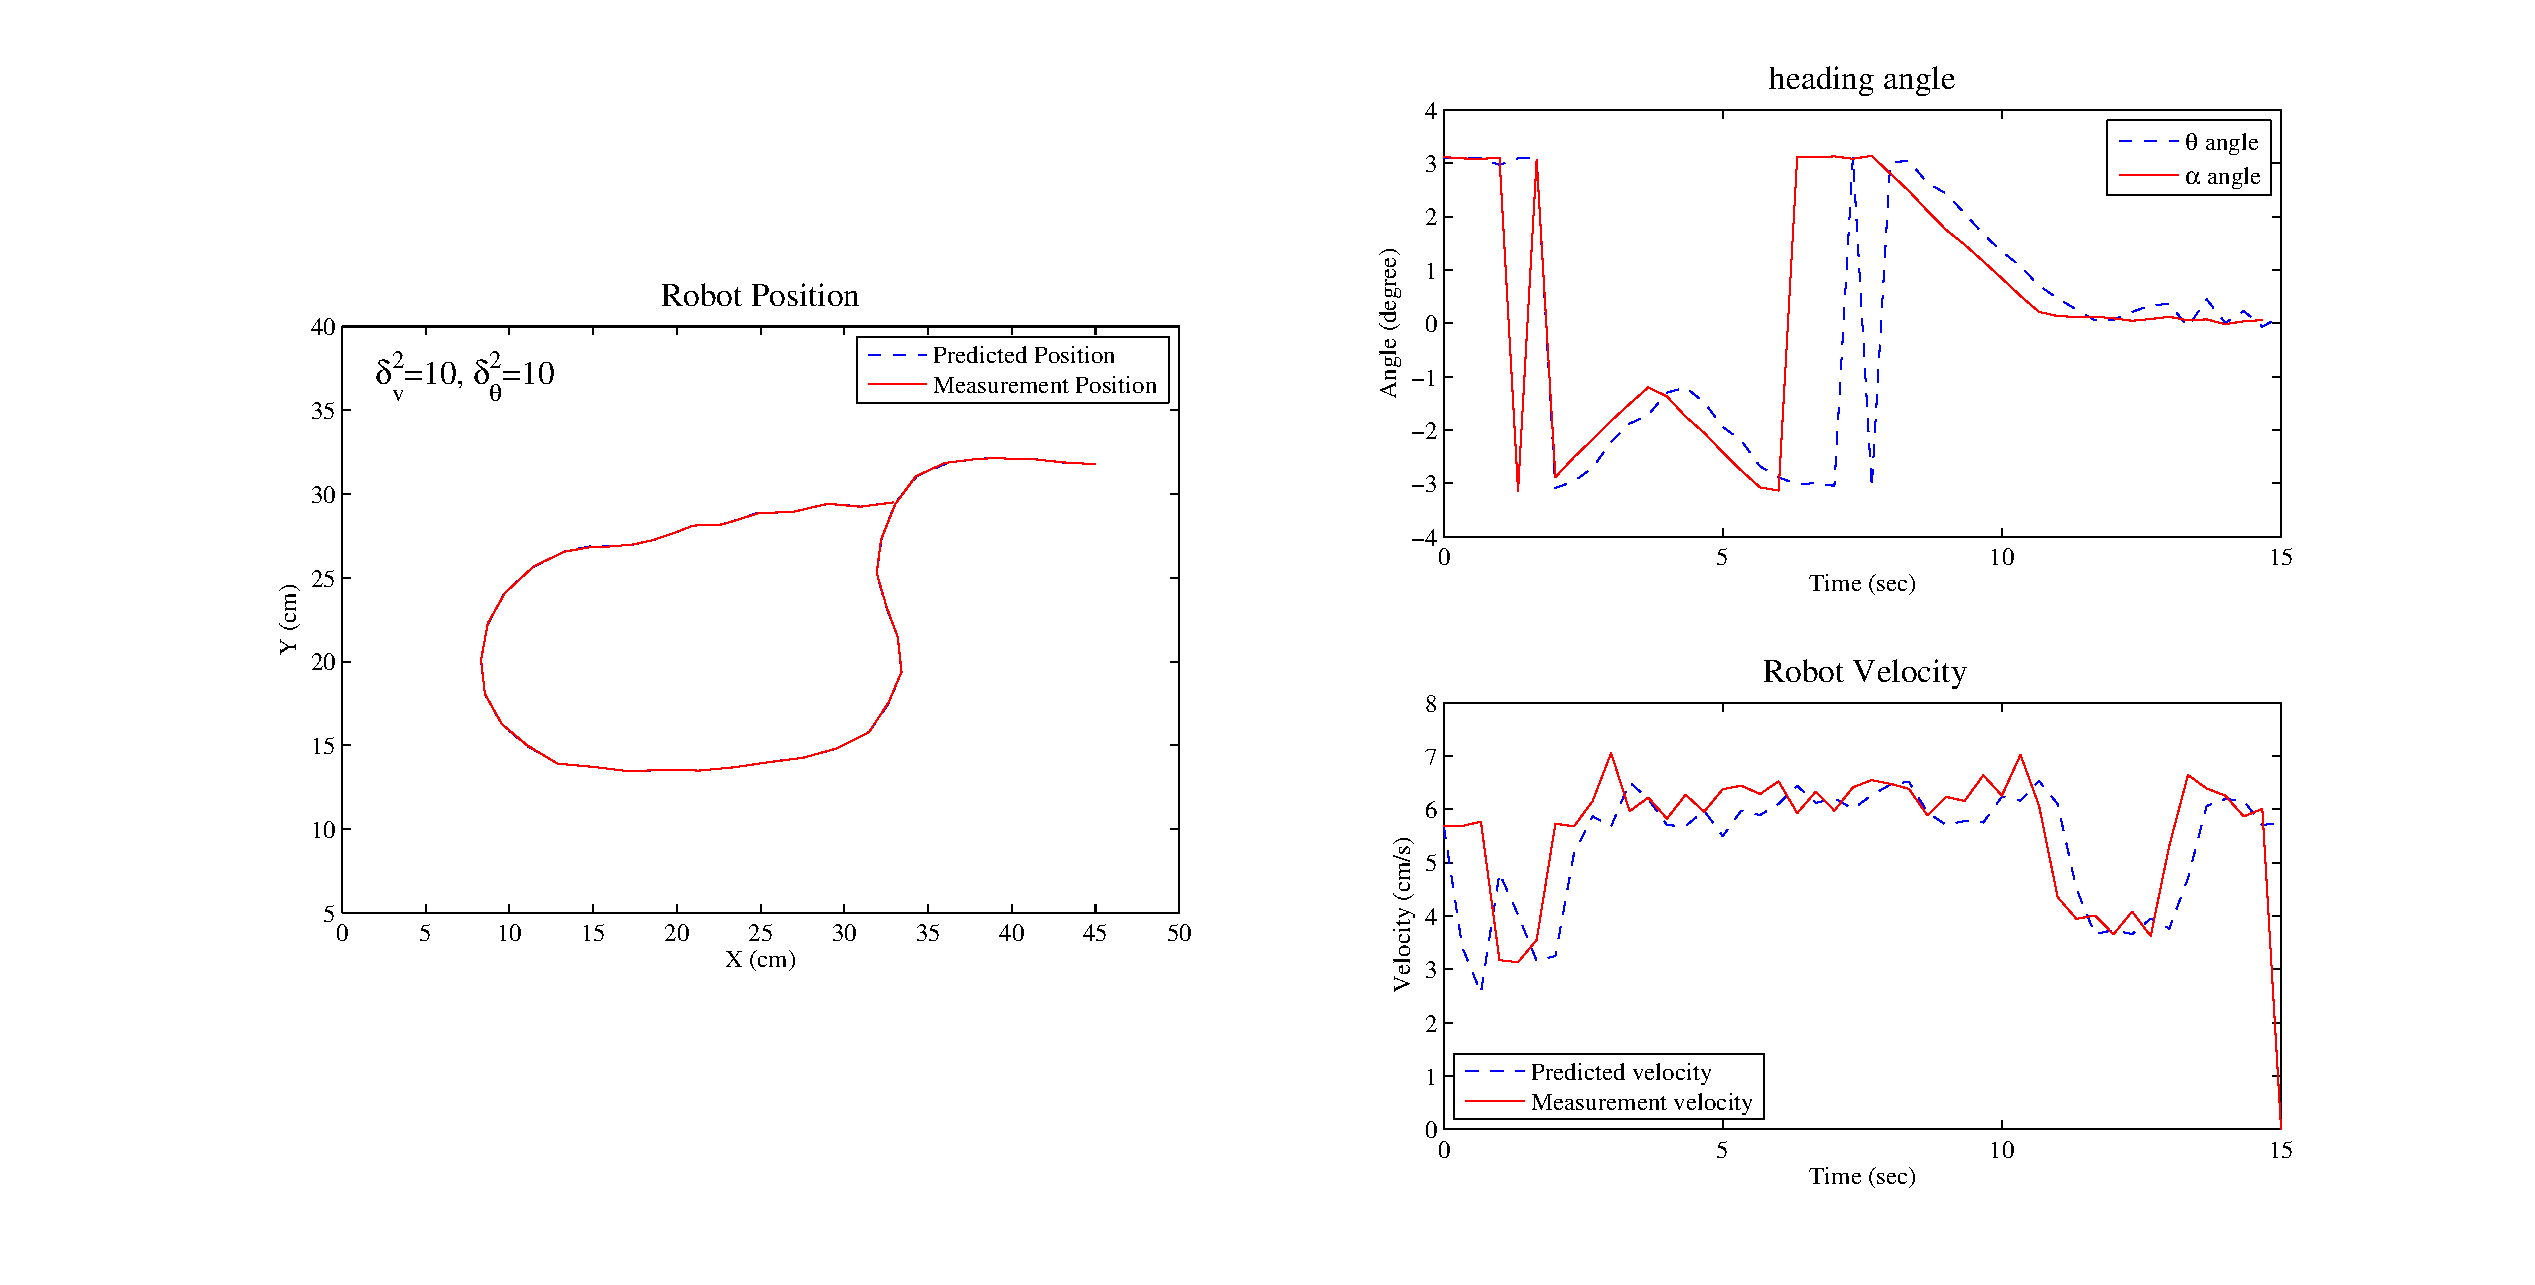
\includegraphics[width=\textwidth]{EKF_v10_w10.eps}
	 	\caption{The result of EKF with $\delta_v^2=10$ and $\delta_\theta^2=10$.}
	 \end{center}
 \end{figure}
 While, in figure 6, it shows that the result of second order filter with larger variance of the process noise ($\delta_v^2=10$ 
 and $\delta_\theta^2=10$) diverge from the measure data. From figure 5 and figure 6, it shows that second order filter 
 is more sensitive to the change of the variance of the process noise. 
 \begin{figure}[H]
	 \begin{center}
	 	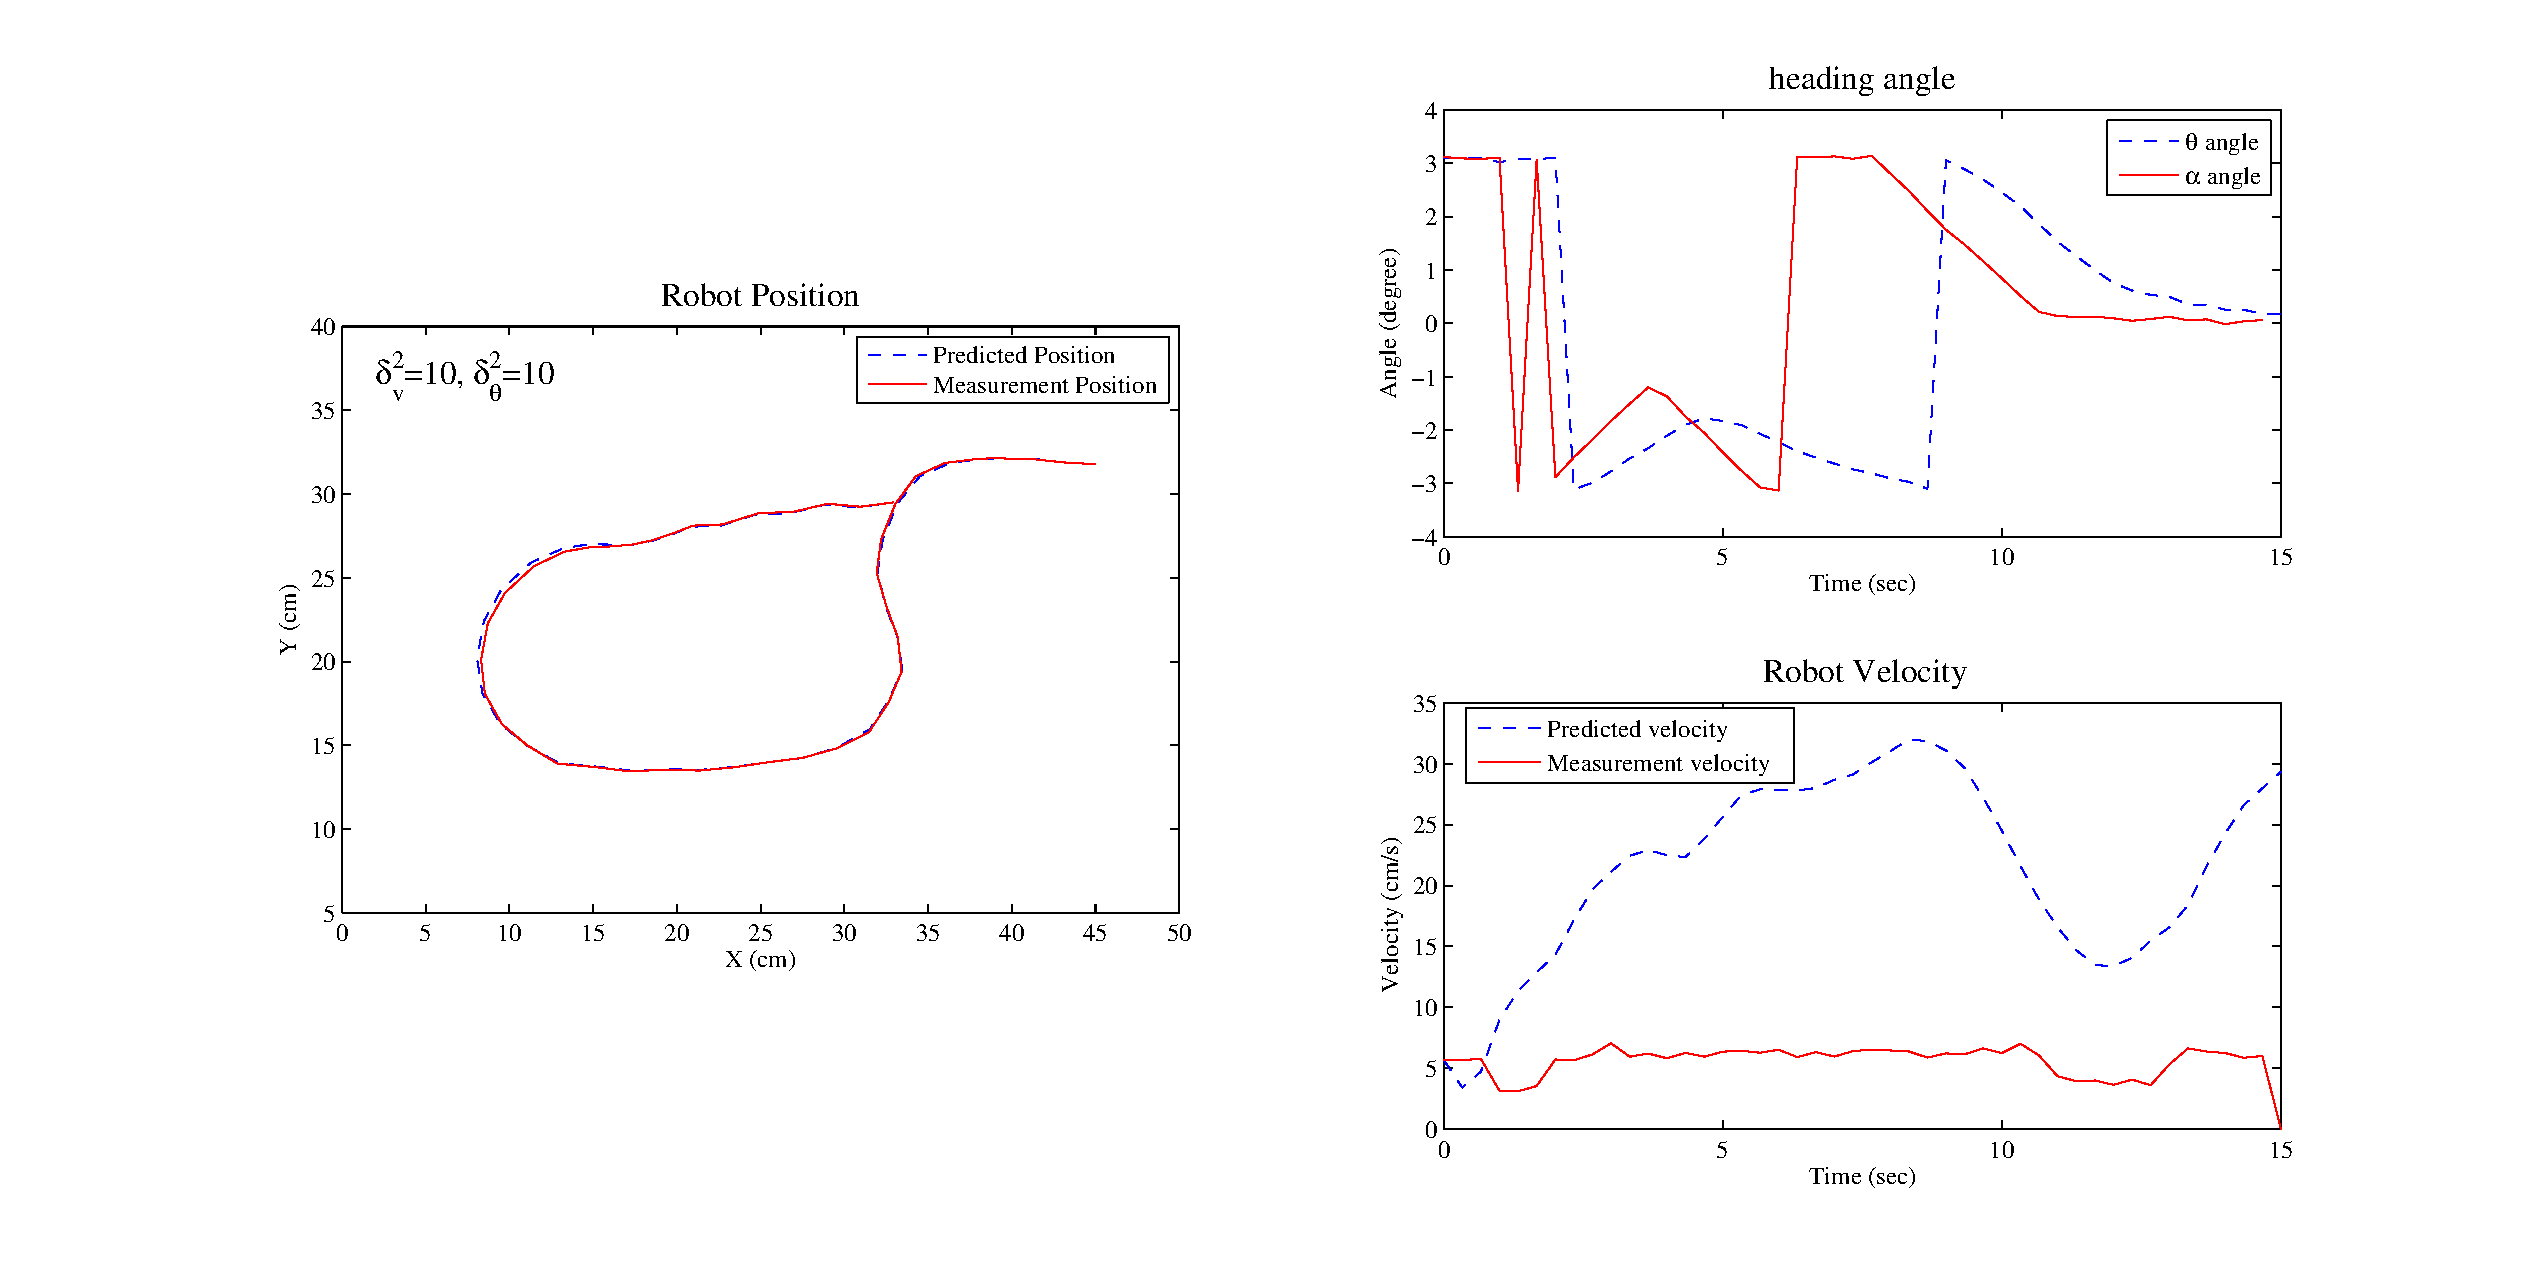
\includegraphics[width=\textwidth]{sof_v10_w10.eps}
	 	\caption{The result of second order filter with $\delta_v^2=10$ and $\delta_\theta^2=10$.}
	 \end{center}
 \end{figure}

\end{document}
